\chapter{Model-to-Text with Moca}

When establishing a model-driven solution, \emph{model transformations} of some sort usually play a central and important role.
Be it for specifying dynamic semantics (like for our memory box) or, more generally, for transforming a certain model to another model to achieve some goal (consistency, adding or abstracting from platform details, \ldots).  

There are many, many different \emph{kinds} of model transformations and \cite{CH03,Mens_Gorp_2006} give a nice and detailed classification along a set of different dimensions. 
Dimensions we shall explore in this chapter include the \emph{source-target relationship} \cite{Mens_Gorp_2006} and if the models involved conform to the same metamodel or not.
We shall also see how \emph{model-to-text} transformations can be achieved with a nice mixture of \emph{string} and \emph{graph grammars}. 

For the rest of the chapter a model transformation is to be regarded as:
\begin{displaymath}
 	\Delta: m_{src} \rightarrow m_{trg}
\end{displaymath}

Where $m_{src}$ is the source model which is to be transformed to $m_{trg}$ the target model.
What we have treated in the tutorial till now were model transformations (SDMs) that manipulated a single model, performing changes directly to the model.
According to \cite{Mens_Gorp_2006} such transformations are \emph{in-place} as $m_{src}$ is destructively changed into $m_{trg}$ and \emph{endogenous} because both versions of the model obviously conform to the same metamodel.
Although this is the natural case for SDMs, \emph{out-place} transformations that produce a separate $m_{trg}$ and do not modify $m_{src}$ can also be specified with SDMs.

\clearpage
To complete the classification and twist your brain a bit here are a few interesting statements:
\begin{quote}
Out-place transformations can be either endogenous or \emph{exogenous} if $m_{src}$ and $m_{trg}$ conform to the same or different metamodels respectively.

In-place transformations can usually\footnote{One can always think up crazy examples right?} only be endogenous.  Exogenous transformations are, consequently, always out-place.  Why? 
\end{quote}  
  

Yet another dimension is if $m_{src}$ and $m_{trg}$ are on the same \emph{abstraction level}.
Depending on if abstraction levels are traversed or not, transformations are classified as being \emph{vertical} or \emph{horizontal}, respectively. 

This abstraction-level dimension is obviously a bit fuzzy and is best understood with a concrete example. 
In this Chapter, we shall complement our memory box with a simple language for \emph{dictionaries}.
A dictionary is also used to learn new words but is more suitable to be used as a reference, i.e., one already knows most of the words and only specific words are looked-up now and then.
A memory box, on the other hand, is more geared towards supporting the actual memorization process.
Ergo?  One could start with a memory box and, when all words have been memorized, transform it to a personalized dictionary for future reference.
If one notices that too many words have been forgotten (typically after a long break or a lazy spell) a dictionary can be transformed \emph{back} to a memory box.
We shall see later on in the chapter that this transformation is actually quite cool as one could, for example, use the history of cards or their difficulty level (fast cards are very simple) to either annotate entries in a dictionary or pre-place cards appropriately in a memory box. 

To make things even more interesting, we shall also establish a textual concrete syntax for our dictionaries and explore how graph transformations can be used, in combination with parser technology and template languages, to implement model-to-text and text-to-model transformations.

\emph{Moca} stands for \emph{Mo}flon \emph{C}ode \emph{A}dapter and refers to (1) the approach we use to integrate string grammars, graph grammars and template languages, (2) how we separate the transformation into different steps, (3) the usage of a generic and simple tree metamodel to consolidate different platforms, and (4) to the framework and tool support that acts as glue to hold all the different parts together.
Fig.~\ref{fig:moca-overview} gives a ``big picture'' of what we plan to achieve in this Chapter.
All explanations are integrated right in the figure so take your time and let it sink in.
We'll be zooming in on bits and pieces in the following sections to make things clearer and more concrete.

%\usepackage{graphics} is needed for \includegraphics
\begin{figure}[htp]
\begin{center}
 \includegraphics[angle=90, height=\textheight]{pics/moca/text-to-model}
  \caption{Overview of model-to-text with the MOCA framework}
  \label{fig:moca-overview}
\end{center}
\end{figure} 


\clearpage

\section{Setup ANTLR}

Install the ANTLR eclipse plugin from \url{http://antlrv3ide.sourceforge.net/updates}

Download ANTLRworks (\url{http://www.antlr.org/works/index.html})
\url{www.antlr.org/download/antlrworks-1.4.3.jar}

%\usepackage{graphics} is needed for \includegraphics
\begin{figure}[!htbp]
\begin{center}
 \includegraphics[width=\textwidth]{pics/moca/0Install/1-antlr-package}
  \caption{ANTLR installation: Builder preferences}
  \label{moca-1-antlr-package}
\end{center}
\end{figure}

Add ANTLR Package:
- Window $>$ Preferences $>$ ANTLR $>$ Builder 
- Choose ``Add'' (see Fig. \ref{moca-1-antlr-package})
- Choose ``Directory'' and browse to the directory with the downloaded
ANTLRworks jar (see Fig. \ref{moca-2-choose-path-to-jar})

%\usepackage{graphics} is needed for \includegraphics
\begin{figure}[!htbp]
\begin{center}
 \includegraphics[width=0.7\textwidth]{pics/moca/0Install/2-choose-path-to-jar}
  \caption{ANTLR installation: dialog for choosing ANTLRworks as builder}
  \label{moca-2-choose-path-to-jar}
\end{center}
\end{figure}




\section{Workspace for Model-to-Text Transformation}

- Start Eclipse with empty Workspace
- Switch to the moflon perspective

%\usepackage{graphics} is needed for \includegraphics
\begin{figure}[!htbp]
\begin{center}
 \includegraphics[width=0.3\textwidth]{pics/moca/1DictionaryMetaModel/1-NewMetamodelWizard}
  \caption{Opening the ``New Metamodel'' wizard}
  \label{moca-1-NewMetamodelWizard}
\end{center}
\end{figure}

- Open the ``New Metamodel'' wizard 

%\usepackage{graphics} is needed for \includegraphics
\begin{figure}[!htbp]
\begin{center}
 \includegraphics[width=0.7\textwidth]{pics/moca/1DictionaryMetaModel/2-AddMocaSupport-ProjectName}
  \caption{Add Metamodel project with MOCA support}
  \label{moca-2-AddMocaSupport-ProjectName}
\end{center}
\end{figure}

- Set project name to ``Dictionary''
- Select "Add Moca Support" 


%\usepackage{graphics} is needed for \includegraphics
\begin{figure}[!htbp]
\begin{center}
 \includegraphics[width=0.3\textwidth]{pics/moca/1DictionaryMetaModel/3-WizardResult}
  \caption{Workspace after wizard finishes}
  \label{moca-3-WizardResult}
\end{center}
\end{figure}

- Project and eap file are created (see Fig. \ref{moca-3-WizardResult})

%\usepackage{graphics} is needed for \includegraphics
\begin{figure}[!htbp]
\begin{center}
 \includegraphics[width=0.5\textwidth]{pics/moca/1DictionaryMetaModel/4-eapContainsMocatreeWithExportFalse}
  \caption{The EA project contains a package ``MocaTree'' with property
  $Moflon::Export = false$}
  \label{moca-4-eapContainsMocatreeWithExportFalse}
\end{center}
\end{figure}

- open Dictionary.eap
- eap file contains MocaTree package with $export = false$ (Fig.
\ref{moca-4-eapContainsMocatreeWithExportFalse})

\begin{figure}[!htbp]
\begin{center}
 \includegraphics[width=\textwidth]{pics/moca/0Install/0-MocaTree}
  \caption{Mocatree metamodel}
  \label{moca-tree}
\end{center}
\end{figure}


%\usepackage{graphics} is needed for \includegraphics
\begin{figure}[!htbp]
\begin{center}
 \includegraphics[width=\textwidth]{pics/moca/1DictionaryMetaModel/5-DictionaryMM}
  \caption{Dictionary metamodel}
  \label{moca-5-DictionaryMM}
\end{center}
\end{figure}

- Add dictionary Metamodel like in (Fig. \ref{moca-5-DictionaryMM})
- Add package ``DictionaryCodeAdapter''

%\usepackage{graphics} is needed for \includegraphics
\begin{figure}[!htbp]
\begin{center}
 \includegraphics[width=0.5\textwidth]{pics/moca/1DictionaryMetaModel/5-DictionaryMM-ProjectBrowser}
  \caption{EA project view before exporting}
  \label{moca-5-DictionaryMM-ProjectBrowser}
\end{center}
\end{figure}

- EA projects just before export (Fig. \ref{moca-5-DictionaryMM-ProjectBrowser}) 

%\usepackage{graphics} is needed for \includegraphics
\begin{figure}[!htbp]
\begin{center}
 \includegraphics[width=0.3\textwidth]{pics/moca/1DictionaryMetaModel/6-ExportToEclipse}
  \caption{Workspace after export to eclipse}
  \label{moca-6-ExportToEclipse}
\end{center}
\end{figure}

- Export to eclipse  (Fig. \ref{moca-6-ExportToEclipse})
 
 
\section{Text-to-Tree Transformation}

As we shall see in a moment, libraries and shelves correspond to a folder structure while the contents for a single dictionary are specified in a file.
Figure \ref{fig:moca-4-Tokens} depicts a small sample of the textual syntax used to specify a dictionary.
On the way to an instance model of our dictionary metamodel, the very first step is to create nice \emph{chunks} of characters.
This is called \emph{lexing} and is a step that simplifies the actual comprehension of the complete text.
Interestingly human beings actually comprehend text in a similar manner, one recognizes whole words without ``seeing'' every individual character.
This is the reason why you can siltl raed tihs sneentce alsomt eforftlsesly.   
A lexer recognizes these chunks or \emph{tokens} and passes them on as a token stream to the \emph{parser} that does the actual work of recognizing complex hierarchical and recursive structures.
   
To recognize the tokens as indicated in Fig.~\ref{fig:moca-4-Tokens}, \texttt{ANTLR} can automatically generate a lexer in Java from a compact specification as depicted in Fig.~\ref{fig:moca-6-lexer}.
This is actually a DSL for lexing and is explained in detail in \cite{ANTLR}.
If you do not know what EBNF is and have problems understanding the lexer grammar then make sure you at least go through the documentation on \url{www.antlr.org} or read relevant chapters in \cite{ANTLR}.

 
%\usepackage{graphics} is needed for \includegraphics
\begin{figure}[!htbp]
\begin{center}
 \includegraphics[width=0.8\textwidth]{pics/moca/2TextToMocaTree/4-tokens}
  \caption{Identified tokens in a dictionary file.}
  \label{fig:moca-4-Tokens}
\end{center}
\end{figure}

\begin{enumerate}
\item[$\blacktriangleright$] Edit \texttt{DictionaryLexer.g} so it closely resembles Fig.~\ref{fig:moca-6-lexer}.
Be careful to avoid any typos and mistakes.  Save and make sure it compiles.  
\end{enumerate}

%\usepackage{graphics} is needed for \includegraphics
\begin{figure}[!htbp]
\begin{center}
 \includegraphics[width=0.75\textwidth]{pics/moca/2TextToMocaTree/6-lexer}
  \caption{Lexer grammar}
  \label{fig:moca-6-lexer}
\end{center}
\end{figure}

The next step is to form the stream of tokens from the lexer into a \emph{tree}.
In this context, a tree is an acyclic, hierarchical, recursive structure as depicted in Fig.~\ref{fig:moca-5-Tree}.
Depending on what the tree is to be used for, it can be structured very differently with \emph{imaginary} nodes like \texttt{DICTIONARY} or \texttt{ENTRY} that were not present in the textual syntax and are used to give additional structure to the tree. 

%\usepackage{graphics} is needed for \includegraphics
\begin{figure}[htp]
\begin{center}
 \includegraphics[width=\textwidth]{pics/moca/2TextToMocaTree/5-tree}
  \caption{MocaTree structure}
  \label{fig:moca-5-Tree}
\end{center}
\end{figure}

\begin{enumerate}
\item[$\blacktriangleright$] Edit \texttt{DictionaryParser.g} so it closely resembles Fig.~\ref{fig:moca-7-parser}.
As with the lexer, avoid typos and mistakes and make sure it compiles.
\end{enumerate}

%\usepackage{graphics} is needed for \includegraphics
\begin{figure}[!htbp]
\begin{center}
 \includegraphics[width=0.9\textwidth]{pics/moca/2TextToMocaTree/7-parser}
  \caption{Parser grammar}
  \label{fig:moca-7-parser}
\end{center}
\end{figure}
The parser grammar is quite similar to the lexer grammar, but there are \emph{parser actions} after \texttt{->} to build up the tree.
Using this simple tree language, one can (1) abstract from tokens like \texttt{\{} or \texttt{\}}, which are just \emph{syntactical noise} and (2) enrich the tree with imaginary nodes like \texttt{ENTRY}, which add explicit structure to the tree.
Please refer to \cite{ANTLR} and online resources for a detailed explanation of the syntax and semantics of the parser grammar supported by \texttt{ANTLR}. 
 
%\usepackage{graphics} is needed for \includegraphics
\begin{figure}[htp]
\begin{center}
 \includegraphics[width=\textwidth]{pics/moca/2TextToMocaTree/8-MocaMain}
  \caption{Generated main method}
  \label{fig:moca-8-MocaMain}
\end{center}
\end{figure}

Before we take our lexer and parser for a spin, open \texttt{MocaMain.java} and inspect it.
If everything went right it should bear a striking resemblance to Fig.~\ref{fig:moca-8-MocaMain}.
For the moment we do not need to adjust anything, just note how the parser is added to the Moca framework (line 23) via an adapter (\texttt{Dictionary\-Parser\-Adapter}).
Go ahead and look at what the adapter exactly does.
All the code can be adjusted and used to, for example, define which files the parser is to be used for (per default the adapter registers for \texttt{*.dictionary} files).
The main job of the adapter is to hide \texttt{ANTLR} specifics so the framework remains (parser) technology agnostic.
If you decide to use a different parser generator or write the parser by hand you would need to implement a corresponding adapter from scratch.

On line 27, the input for the framework is set, meaning that all folders in \texttt{./instances/in} are parsed.
In a nutshell, each folder is taken as a root of a tree and the folder and file structure is reflected as a hierarchy of (children)nodes in the tree.
For each file, the framework searches for a registered parser that is responsible for the particular file, passes the content on to the parser and plugs in the tree from the parser as a single subtree of the corresponding file node in the overall tree.  Take a look at Fig.~\ref{fig:moca-overview} again and review the parts we have covered.

The final step is to prepare some input for the framework:

\begin{enumerate}
  \item[$\blacktriangleright$] Create the directory structure in \texttt{./instances/in} as depicted in Fig.~\ref{fig:moca-inputdata}.  Create each \texttt{dictionary} file as indicated and enter the contents from Fig.~\ref{fig:moca-inputfiles}.
  
  %\usepackage{graphics} is needed for \includegraphics
\begin{figure}[htp]
\begin{center}
  \includegraphics[width=\textwidth]{pics/moca/2TextToMocaTree/inputData}
  \caption{Input directory structure.}
  \label{fig:moca-inputdata}
\end{center}
\end{figure}
  
  %\usepackage{graphics} is needed for \includegraphics
\begin{figure}[htp]
\begin{center}
  \includegraphics[width=0.4\textwidth]{pics/moca/2TextToMocaTree/inputFiles1}
  \includegraphics[width=0.4\textwidth]{pics/moca/2TextToMocaTree/inputFiles2}
  \caption{Input files containing dictionaries.}
  \label{fig:moca-inputfiles} 
\end{center}
\end{figure}
  
  \item[$\blacktriangleright$] Run \texttt{MocaMain.java} as a normal Java application. If everything works out right, a \texttt{tree.xmi} and an \texttt{out} folder should be created in \texttt{instances}.  Inspect their contents and compare to Fig.~\ref{fig:moca-9-ParseResult1}. The unparsed files are obviously empty as we haven't implemented an \emph{unparser} yet.  We shall get to this later on in the chapter.
%\usepackage{graphics} is needed for \includegraphics
\begin{figure}[htp]
\begin{center}
 \includegraphics[width=0.5\textwidth]{pics/moca/2TextToMocaTree/9-ParseResult1}
  \caption{Directory \texttt{instances} after parsing}
  \label{fig:moca-9-ParseResult1}
\end{center}
\end{figure}
  \item[$\blacktriangleright$] Double-click \texttt{tree.xmi}\footnote{Depending on the plugins you have installed, you might have to explicitly choose \texttt{Open With/Sample Reflective Ecore Model Editor}.} and compare the contents to Fig.~\ref{fig:moca-10-ParseResult2}. At this point, you can reflect on the structure of the tree and note the directory structure, file nodes and the subtrees from the parser.
%\usepackage{graphics} is needed for \includegraphics
\begin{figure}[htp]
\begin{center}
 \includegraphics[width=0.5\textwidth]{pics/moca/2TextToMocaTree/10-ParseResult2}
  \caption{MocaTree created by Parser}
  \label{fig:moca-10-ParseResult2}
\end{center}
\end{figure}
\end{enumerate}

If everything worked out then well done!  We now have a nice tree that we can work on with SDMs and transform in a few simple steps to an actual instance of our Dictionary metamodel.

%%\usepackage{graphics} is needed for \includegraphics
\begin{figure}[!htbp]
\begin{center}
 \includegraphics[width=\textwidth]{pics/moca/3MocaTreeToModel/DictionaryCodeAdapter}
  \caption{Dictionary CodeAdapter}
  \label{fig:moca-DictionaryCodeAdapter}
\end{center}
\end{figure}


%\usepackage{graphics} is needed for \includegraphics
\begin{figure}[!htbp]
\begin{center}
 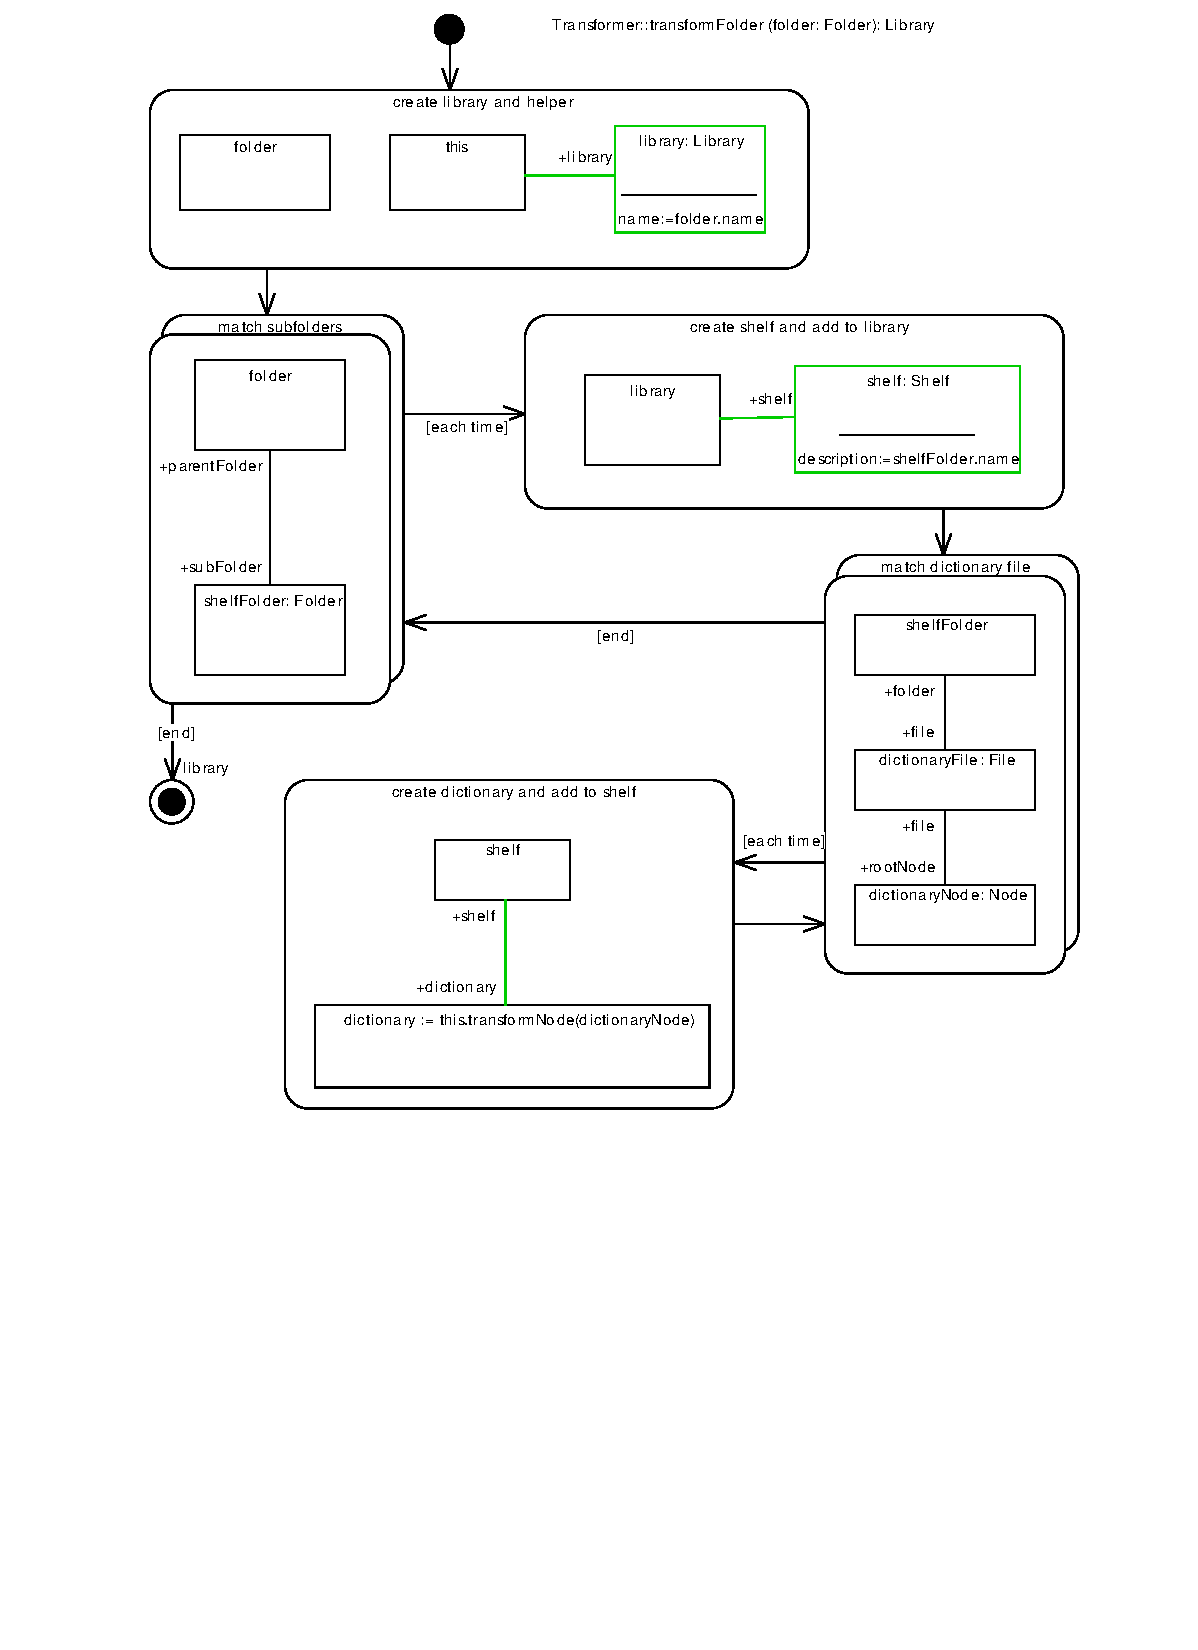
\includegraphics[width=\textwidth]{pics/moca/3MocaTreeToModel/transformFolderPrintPdf}
  \caption{SDM transformFolder}
  \label{fig:moca-transformFolder}
\end{center}
\end{figure}

%\usepackage{graphics} is needed for \includegraphics
\begin{figure}[!htbp]
\begin{center}
 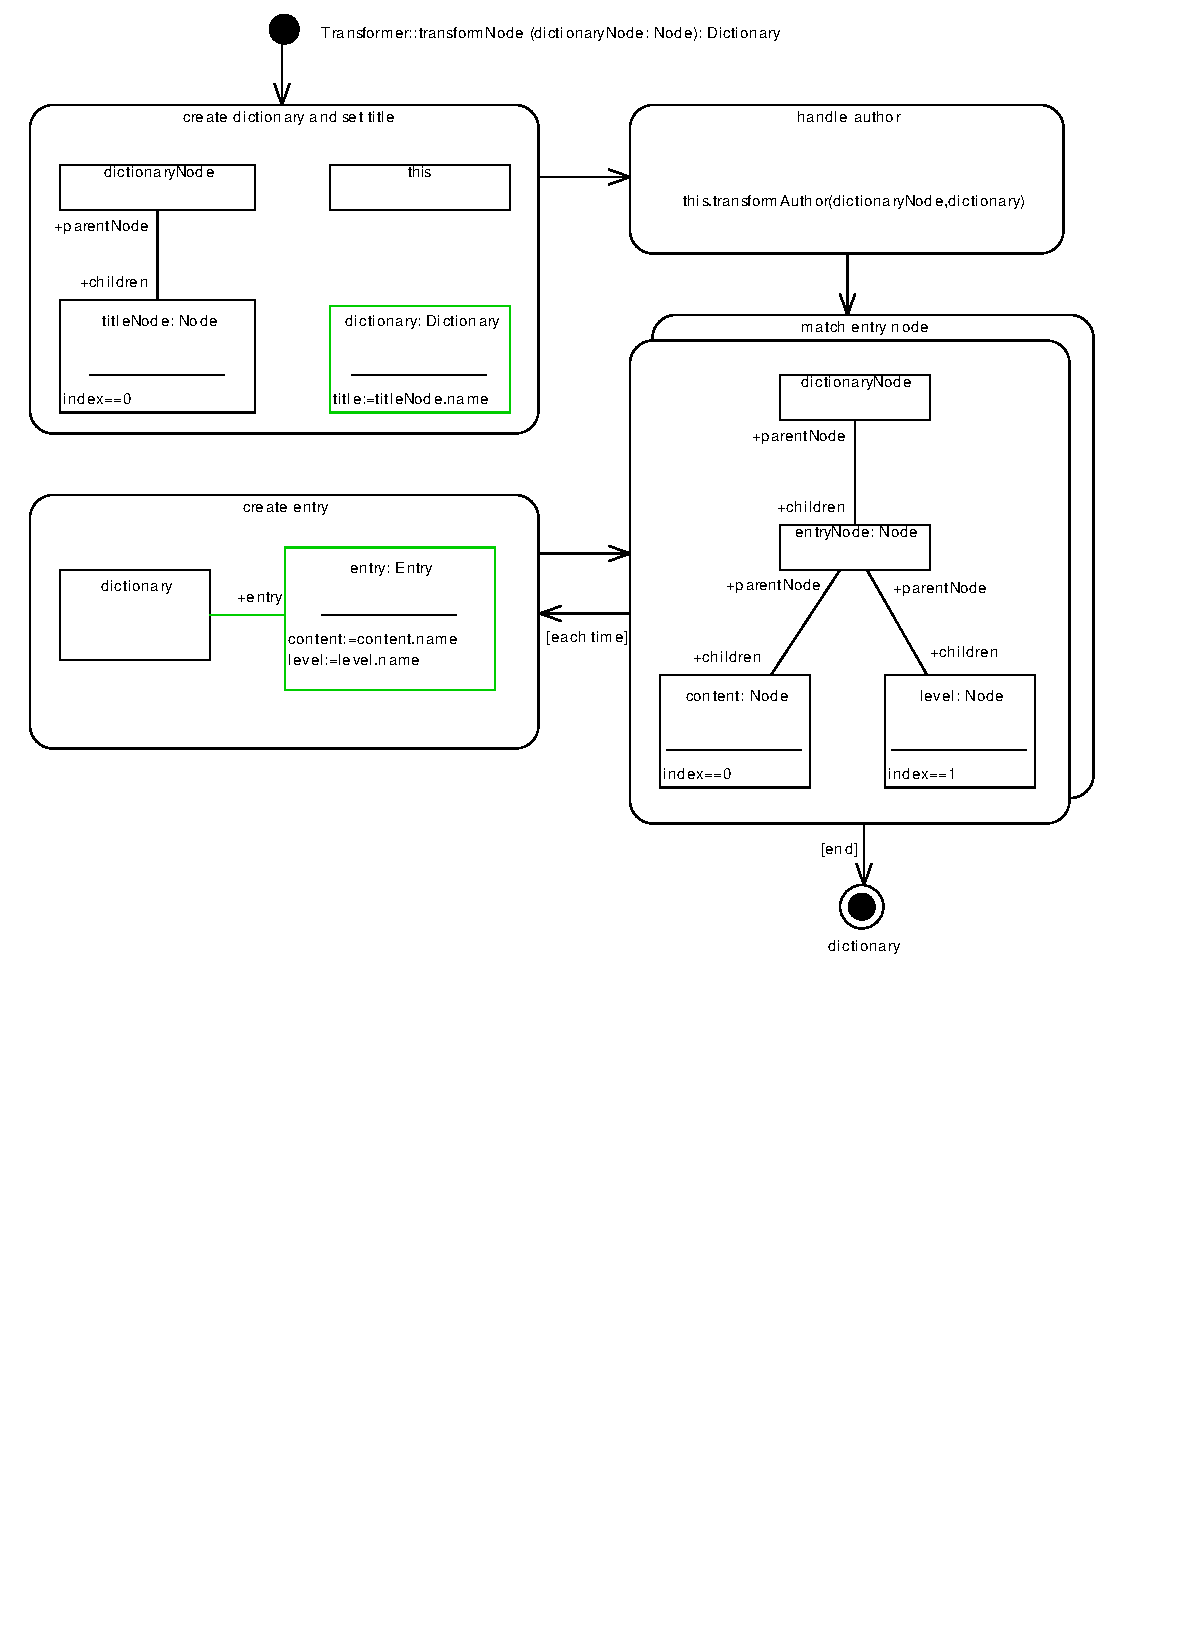
\includegraphics[width=\textwidth]{pics/moca/3MocaTreeToModel/transformNodePrintPdf}
  \caption{SDM transformNode}
  \label{fig:moca-transformNode}
\end{center}
\end{figure}

%\usepackage{graphics} is needed for \includegraphics
\begin{figure}[!htbp]
\begin{center}
 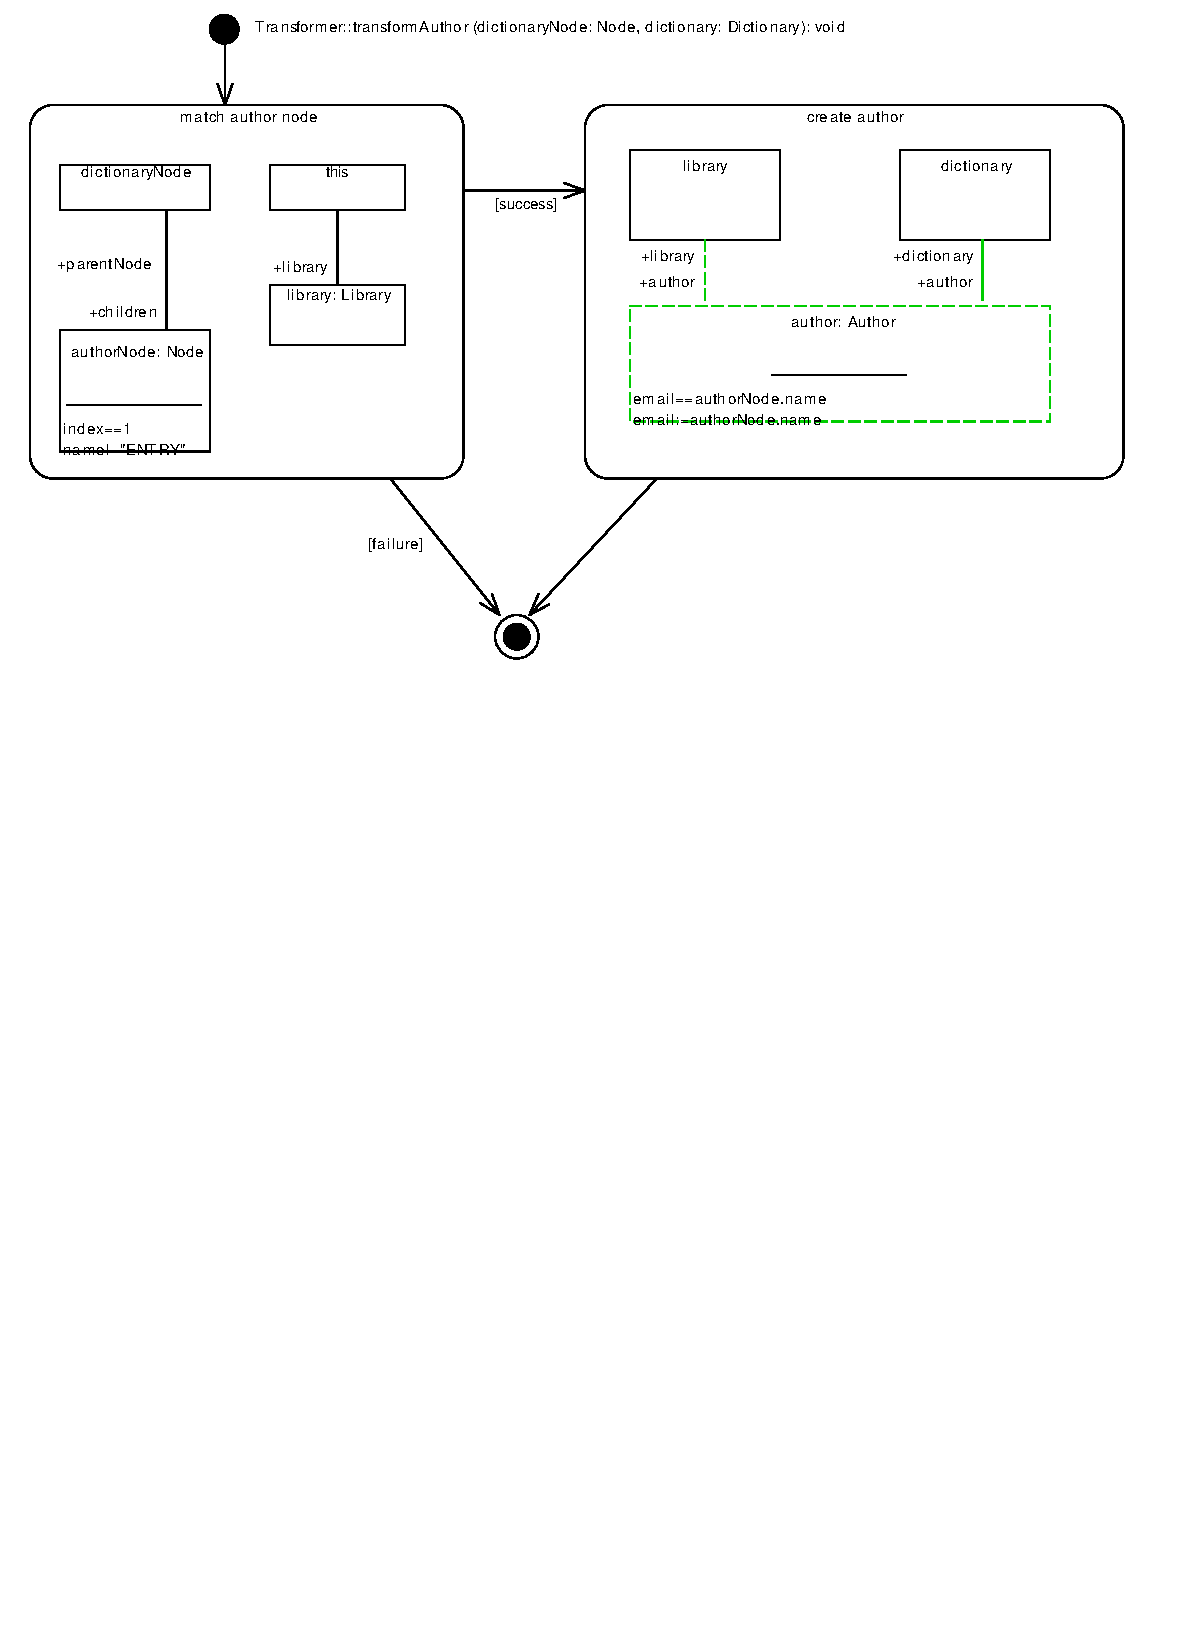
\includegraphics[width=\textwidth]{pics/moca/3MocaTreeToModel/transformAuthorPrintPdf}
  \caption{SDM transformAuthor}
  \label{fig:moca-transformAuthor}
\end{center}
\end{figure}


%\input{mocaHTML}
 
